

\section{Project Objective}

The objective of project is to understand the task of Natural Language Inference in Natural Language Processing.
Natural Language Inference deals with understanding the relationship between 2 given sentences. It tries to identify whether a given sentence, called as \textbf{\textit{"Hypothesis"}} can be derived/inferred/deduced from another given sentence, called \textbf{\textit{"Premise"}} or not. The relationship can be classified into 3 different classes/labels – \par
\begin{itemize}
	\item \textbf{Contradiction} – refers to a situation when both, premise and hypothesis, cannot be true at the same time.
	\item \textbf{Entailment} - refers to a situation where Hypotheses can be derived/inferred from given premise.
	\item \textbf{Neutral} – refers to a situation where there is not enough information in premise to infer or derive the given hypothesis.
\end{itemize}


\section{About Datasets}
For this task, we have explored the 2 famous available datasets – SNLI and Multi NLI.

\subsection{SNLI}
SNLI stands for Stanford Natural Language Inference. It is a benchmark dataset for natural language inference tasks.
\begin{itemize}
	\item All the premises are the image captions from Flicker30 dataset and hence it makes SNLI somewhat genre restricted.
	\item All the hypotheses are written by Crowd-workers i.e., corresponding to a premise, crowd workers will write 3 sentences one for each class.
	\item Total of 550152 train examples with 10,000 as dev samples and 10,000 as test samples, balanced equally across 3 classes.
	\item Mean token length in SNLI dataset i.e., the average number of words per sentence
	\begin{itemize}
		\item For premise - 12.9 
		\item For hypothesis - 7.4
	\end{itemize}
	\item Approximately 56, 951 examples are validated by 4 additional annotators with 91.2\% of gold labels matched with author’s labels.
	\item For SNLI dataset the overall Fleiss' kappa is 0.70, which is defined as the degree of agreement between the annotators, based both categorical labels and similarity matrix.
	\item Progress on SNLI dataset for Natural Language Inference task
	\begin{itemize}
		\item Red line indicates the human performance on SNLI dataset
	\end{itemize}
	\end{itemize}
	
	\begin{figure}[h]
		\centering
		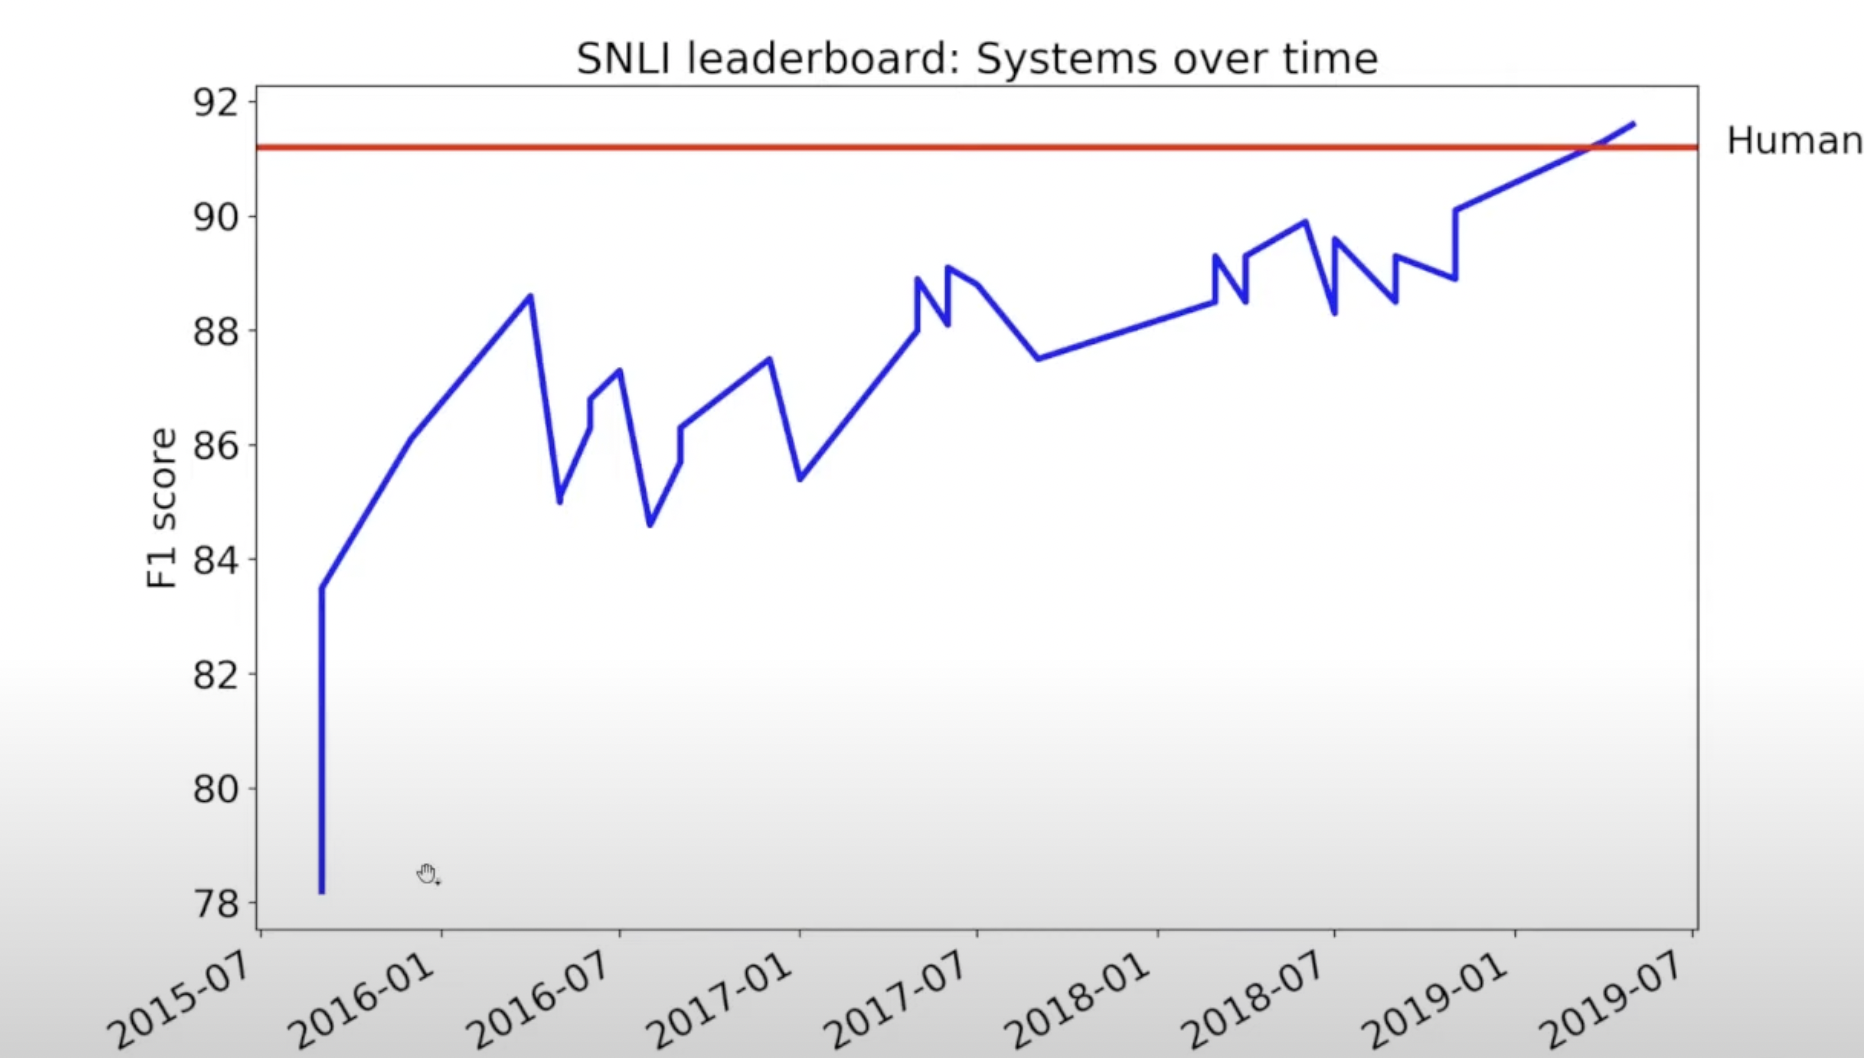
\includegraphics[scale=0.5]{img/snli.png}
		\caption{SNLI Leaderboard \cite{ytvid}}
	\end{figure}
	
	\textit{The main fundamental logic in SNLI is – relating to image dataset, if premise and hypothesis probably describe a different photo, then the label is a contradiction.}

\subsection{MultiNLI}

MultiNLI stands for Multi-Genre Natural Language Inference. It is also another benchmark dataset for natural language inference tasks. It is an extension of the SNLI dataset, with a more diverse set of genres and sources and hence making it a more challenging dataset to train and evaluate the NLI models.
\begin{itemize}
	\item Train Premises in MultiNLI are contributed from 5 genres
	\begin{itemize}
		\item Fiction: works from 1912 – 2010 : spanned across many genres.
		\item Govt. information – available public reports, letters, speeches, Govt. websites etc.
		\item The Slate website
		\item The Switchboard corpus – Telephonic conversation
		\item Bertlitz travel guide
	\end{itemize}
	\item In addition to above genres, premises from some other genres are also present in dev and test datasets like
	\begin{itemize}
		\item From 9/11 reports
		\item From fundraising letters
		\item Nonfiction from Oxford University Press
		\item Verbatim – articles about linguistics.
	\end{itemize}
	\item Total of approx. 3,92,702 train examples with 20,000 as dev samples and 20,000 as test samples.
	\item Approx. 19,647 samples are validated by 4 additional annotators with 92.6\% of gold labels matched with author’s labels.
	\item Test dataset of MultiNLI is only available on Kaggle and in the form of competition.
	\item Progress on SNLI dataset for Natural Language Inference task
	\begin{itemize}
		\item Red line indicates the human performance on Multi NLI dataset
	\end{itemize}
\end{itemize}

\begin{figure}[h]
	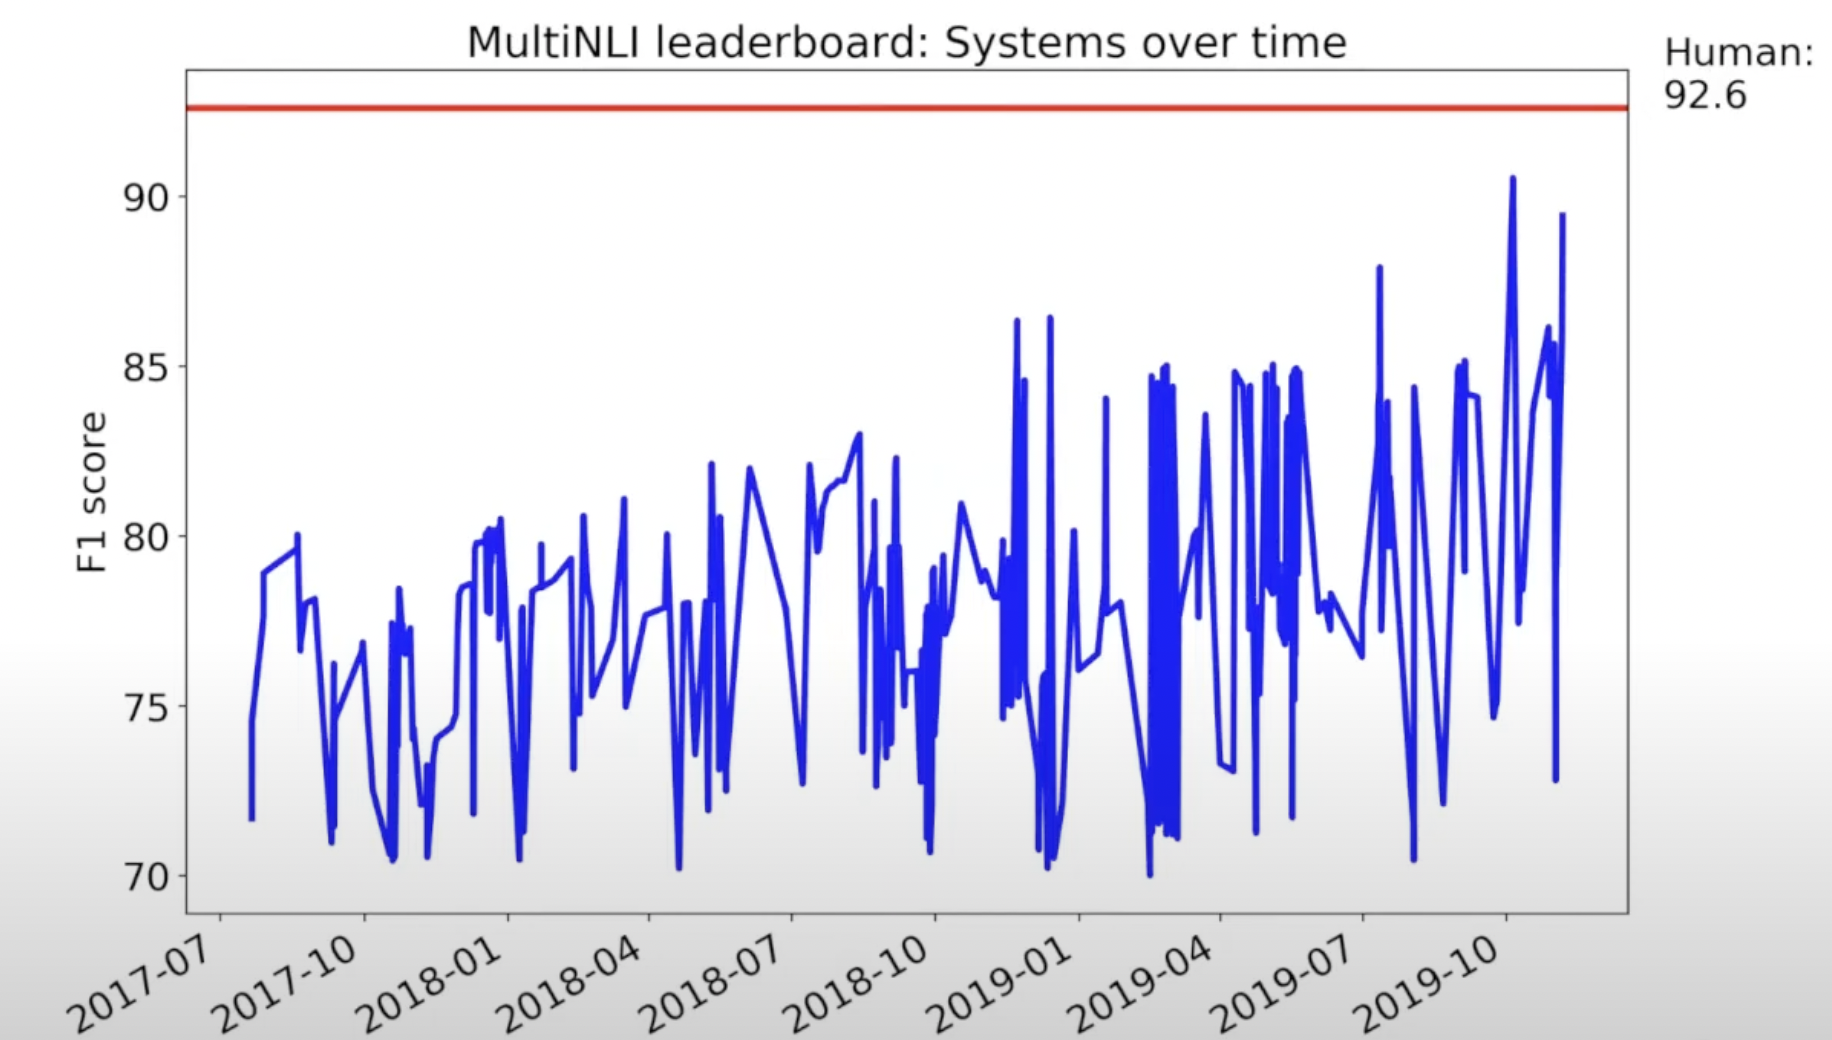
\includegraphics[scale=0.5]{img/multinli.png}
	\caption{MultiNLI Leaderboard \cite{ytvid}}
\end{figure}


There is so much variance in MultiNLI progress as compared to SNLI dataset because MultiNLI dataset is available on Kaggle and so there are too much data points/model to compare. But in SNLI, the progress is reported only from the implemented research papers only and not some from public domain, which is the case in MultiNLI.

\textit{The MultiNLI dataset is filled with distributed annotations that help to perform out of the box error analysis.}


For our further work, we have chosen the SNLI dataset because for SNLI, the test dataset is available and can be easily downloaded. In case of MultiNLI, test data is available only on Kaggle and in the form of competition and hence it cannot be downloaded. Thus after training the models we will be trying them out on the MultiNLI dataset as well.

